\chapter{LLVM}
\section{History}
\begin{wrapfigure}{l}{.5\textwidth}
    \caption[The logo of LLVM]{The logo of LLVM \cite{llvmLogo}}
    
\includegraphics[width=.5\textwidth]{gfx/llvmLogo.png}
\end{wrapfigure}
The \llvm is a collection of modular and reusable compiler and toolchain technologies to support of static and dynamic Compilation as well as tranparent and lifelong program analysis and transformations of arbitrary programs. \cite{LLVMWebsite, LLVMResearchBeginning}\\
The \llvm former was a reasearch project at the university of Illinois, which was first described in a publication in 2004.\draftnote{TODO: Think about sentence}
The project was getting so popular that in 2014 the \llvm Foundation was founded for organizing and maintaining the project. \cite{LLVMFoundation}\\
In order to make the \llvm as independent as possible of the programming language used, the \llvmir was created which is solely used within the pipeline.
\enquote{\llvmir is a strongly typed, \ac{SSA} language that connects to a wide variety of high-level languages.} \cite{PolyhedralEmpiricalStudy}

\section{Pipeline}
The pipeline of the \llvm (\autoref{fig:llvmPipeline}) translates files containing sourcecode written in an arbitrary programming language into \llvmir, on which the following components operate.
At the end assembler is generated out of the (possibly) newly formed \llvmir by the \generator. \cite{IntroLLVM}
\begin{figure}[!ht]
    \caption{The pipeline of LLVM}
    \label{fig:llvmPipeline}
    \centering
    \begin{tikzpicture}
        \node(languages)[nonLlvmIrNode]{C/C++/Obj-C};
        \node(clang)[nonLlvmIrNode, right=of languages]{clang frontend};
        \node(opt)[llvmIrNode, right=of clang]{\opt};
        \node(generator)[llvmIrNode, below=of opt]{\generator};
        \node(linker)[nonLlvmIrNode, left=of generator]{\linker};
        \path[nonLlvmIrPath] (languages) to (clang);
        \path[llvmIrPath] (clang) to (opt);
        \path[llvmIrPath] (opt) -| ($(opt.north east) + (0.5,0.5)$) -| node[auto]{Pass} (opt);
        \path[llvmIrPath] (opt) to (generator);
        \path[nonLlvmIrPath] (generator) to (linker);
    \end{tikzpicture}
    \legend
\end{figure}\\
\subsection{clang frontend}\label{subsec:clangfrontend}
More precisly files containing sourcecode are translated by the clang frontend -- currently at least C, C++ and languages based on C are supported -- into \llvmir by adding the option \texttt{-emit-llvm} \enquote{to abstract away from the specifics} \cite{FastScopDetection} of a programming language.
The option \texttt{-S} can be passed to generate a human readable textfile instead of a \llvmir binary.
\subsection{LLVM Optimizer}\label{subsec:optimizer}
On the received files the \opt can perform steps optimizing and analysing the code.
These steps are called \enquote{Passes}.
These can be explicitly added by specifying appropriate options to the command \texttt{opt} of the \opt.
The option \texttt{-S} can also be specified for generating a human readable textfile like in \autoref{subsec:clangfrontend}.\\
It is also possible to add further options by loading multiple libraries using the flag \texttt{-load}.
\subsection{LLVM Code Generator}
When all desired passes are performed the \generator translates the \llvmir into assembler.
\subsection{LLVM Linker}
The \linker finally compiles an executable binary.
\subsection{Control Flow Graph (CFG)}
\begin{wrapfigure}{l}{.3\textwidth}
    \caption{The CFG of \autoref{lst:matmulll}}
    \label{fig:exampleCfg}
    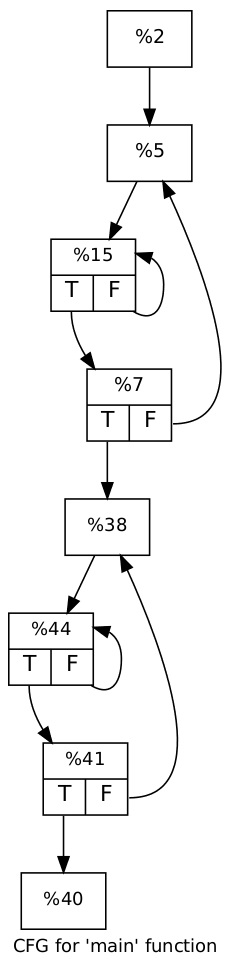
\includegraphics[height=12cm]{gfx/matmulCfg.png}
\end{wrapfigure}
At any point the current \cfg of a \llvmir file can be visualized (like \autoref{fig:exampleCfg}) by passing one of the options \texttt{-view-cfg} or \texttt{-view-cfg-only} to opt.
The \cfg is used by many analysis passes for determining which optimizations can or should be applied.
